\subsection{Problem Setting}

% \begin{frame}
% \frametitle{Problem Setting}
% 
% \begin{columns}
% 	\begin{column}{0.5\textwidth}
% 		\only<1>{ 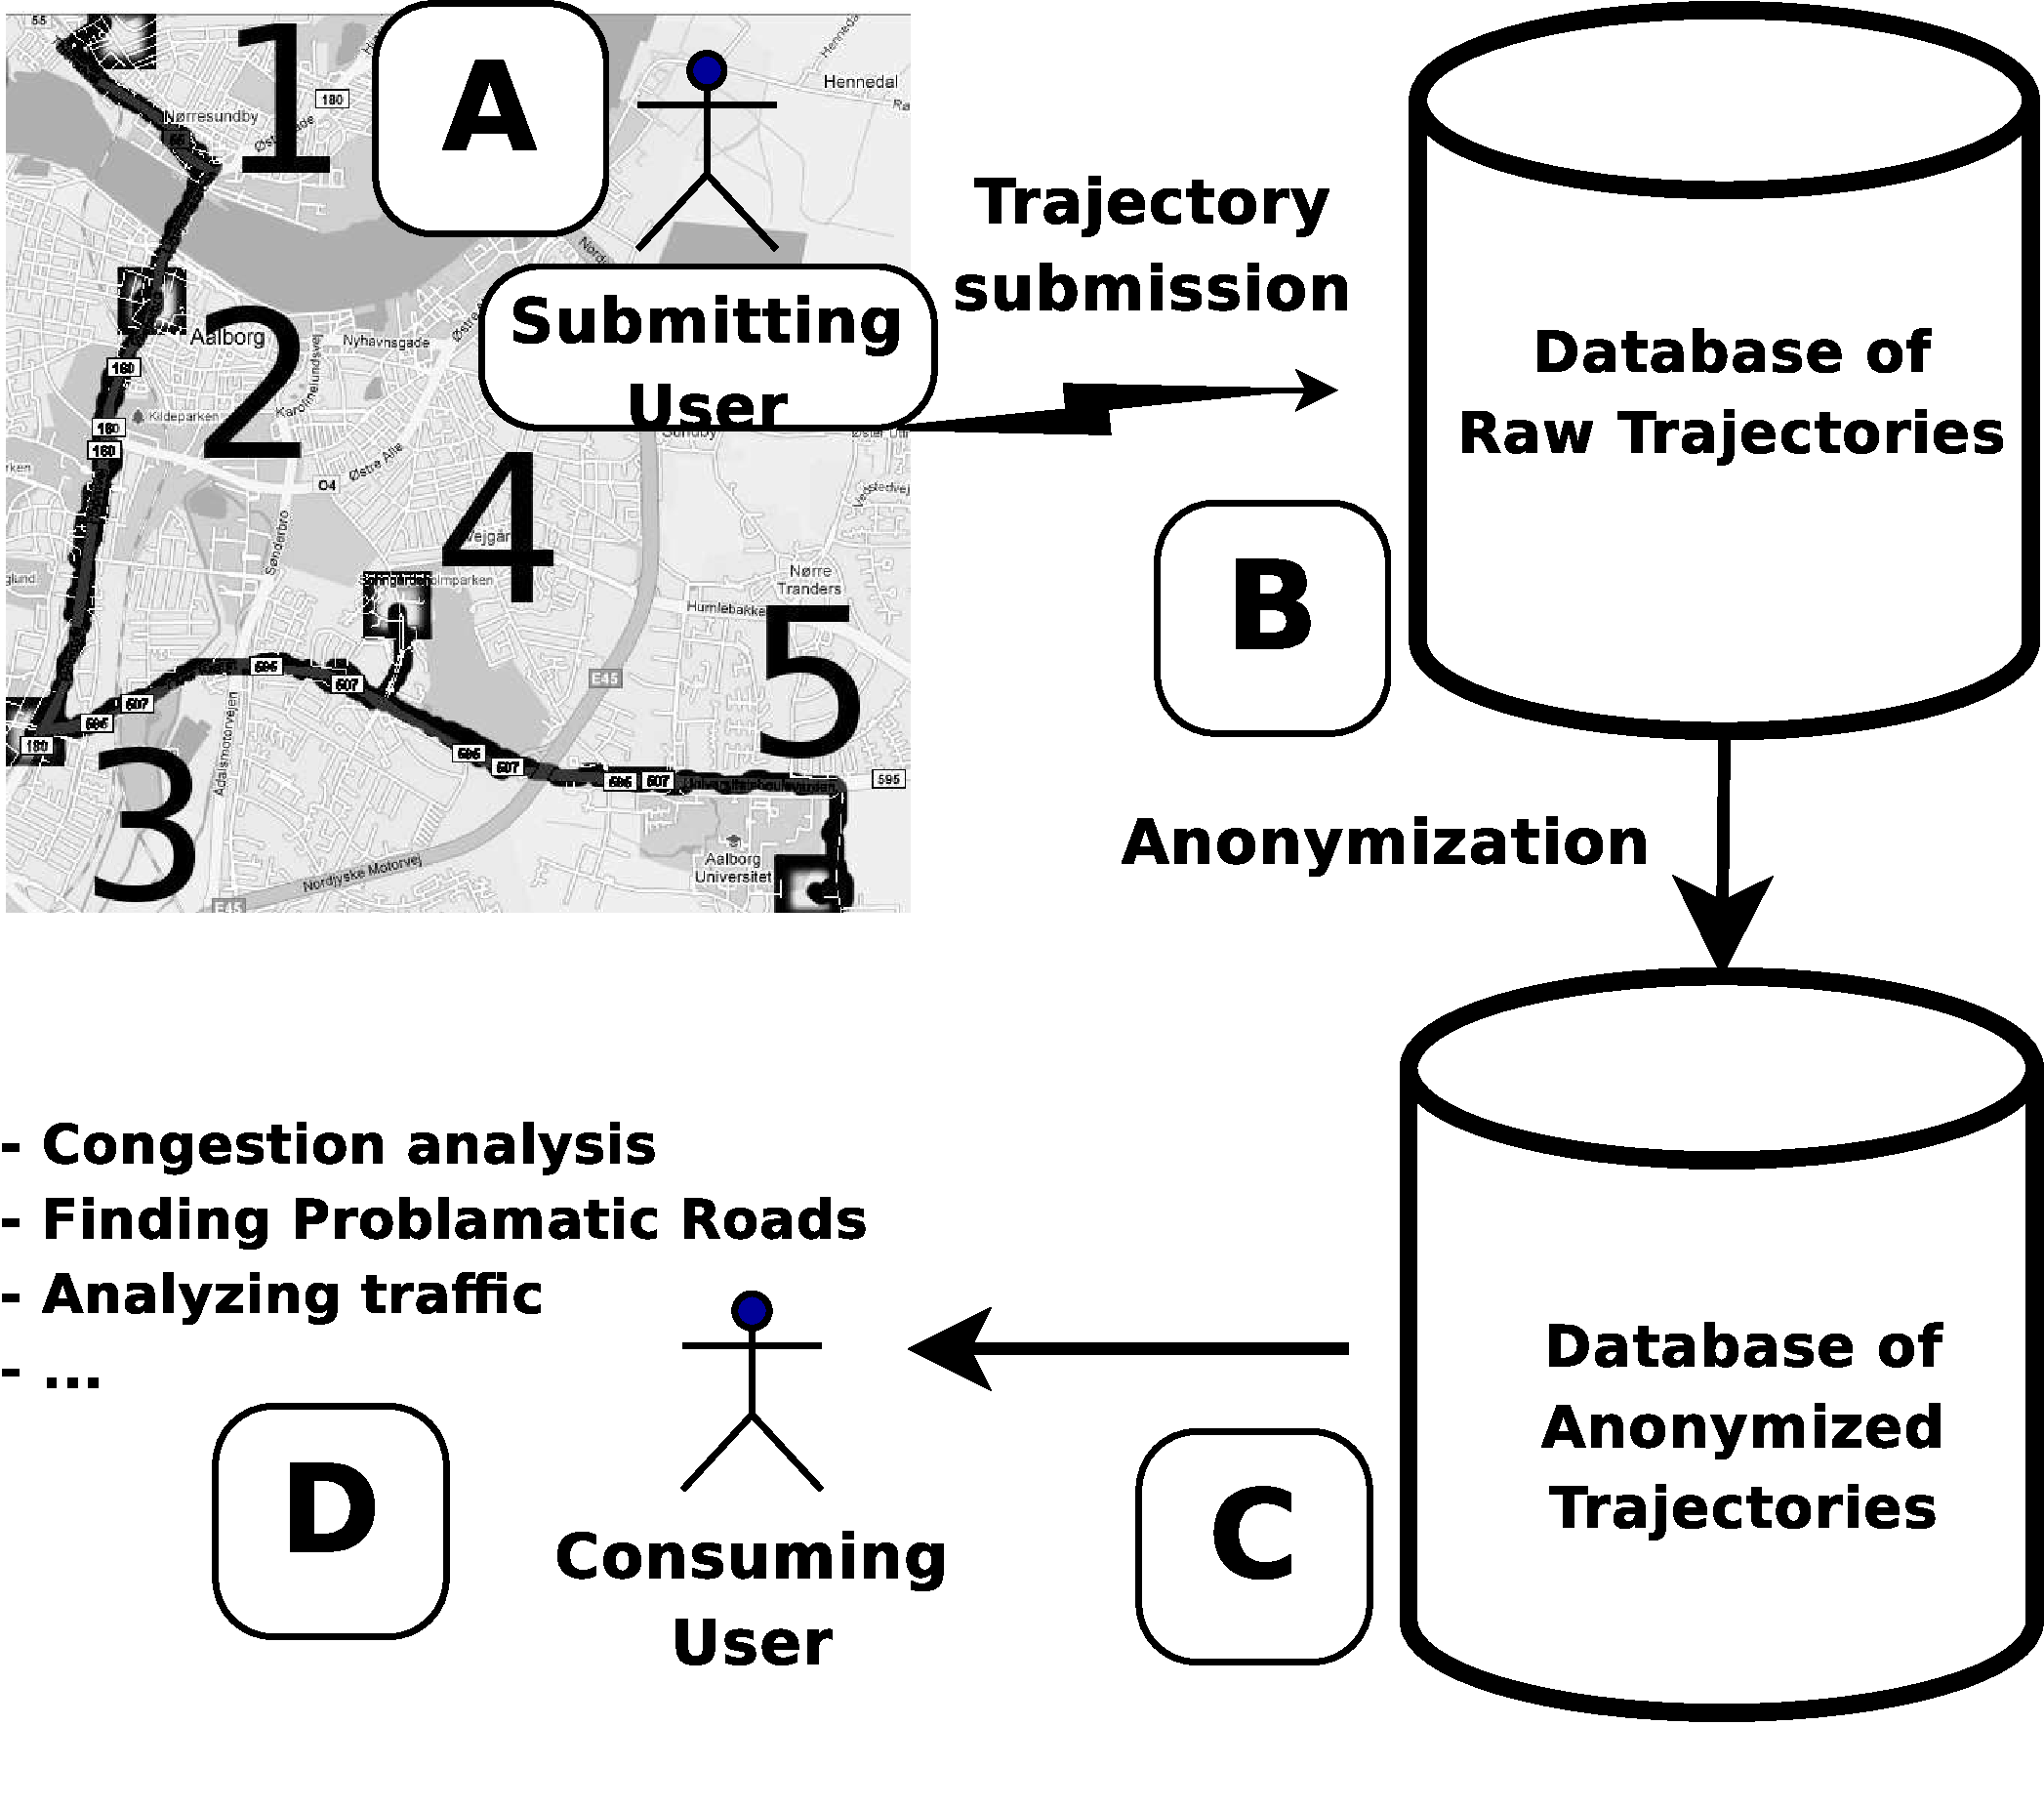
\includegraphics[page=1,scale=0.2]{images/overview.pdf}}
% 	\end{column}
% 	\begin{column}{0.5\textwidth}
% 		\begin{description}\itemsep 16pt
% 		\item[A] Privacy Aware User
% 		\item[B] Trusted Server
% 		\item[C] Public Untrusted Server
% 		\item[D] Service Providers
% 		\end{description}
% 	\end{column}
% \end{columns}
% \end{frame}


%\begin{figure}
%\includegraphics[scale=0.5]{images/prez2.pdf} 
%\caption{show an example picture}
%\end{figure}
%\begin{theorem}
%  In a right triangle, the square of hypotenuse equals
%  the sum of squares of two other sides.
%\end{theorem}

%  Things in a Bulleted List\pause
%  \begin{itemize}
%  \item Bullets that\pause
%  \item Come up\pause
%  \item One by one %leave out the \pause on the final item
%  \end{itemize}
  
